\documentclass{standalone}
\usepackage{tikz}
\usetikzlibrary{patterns, positioning}


\begin{document}
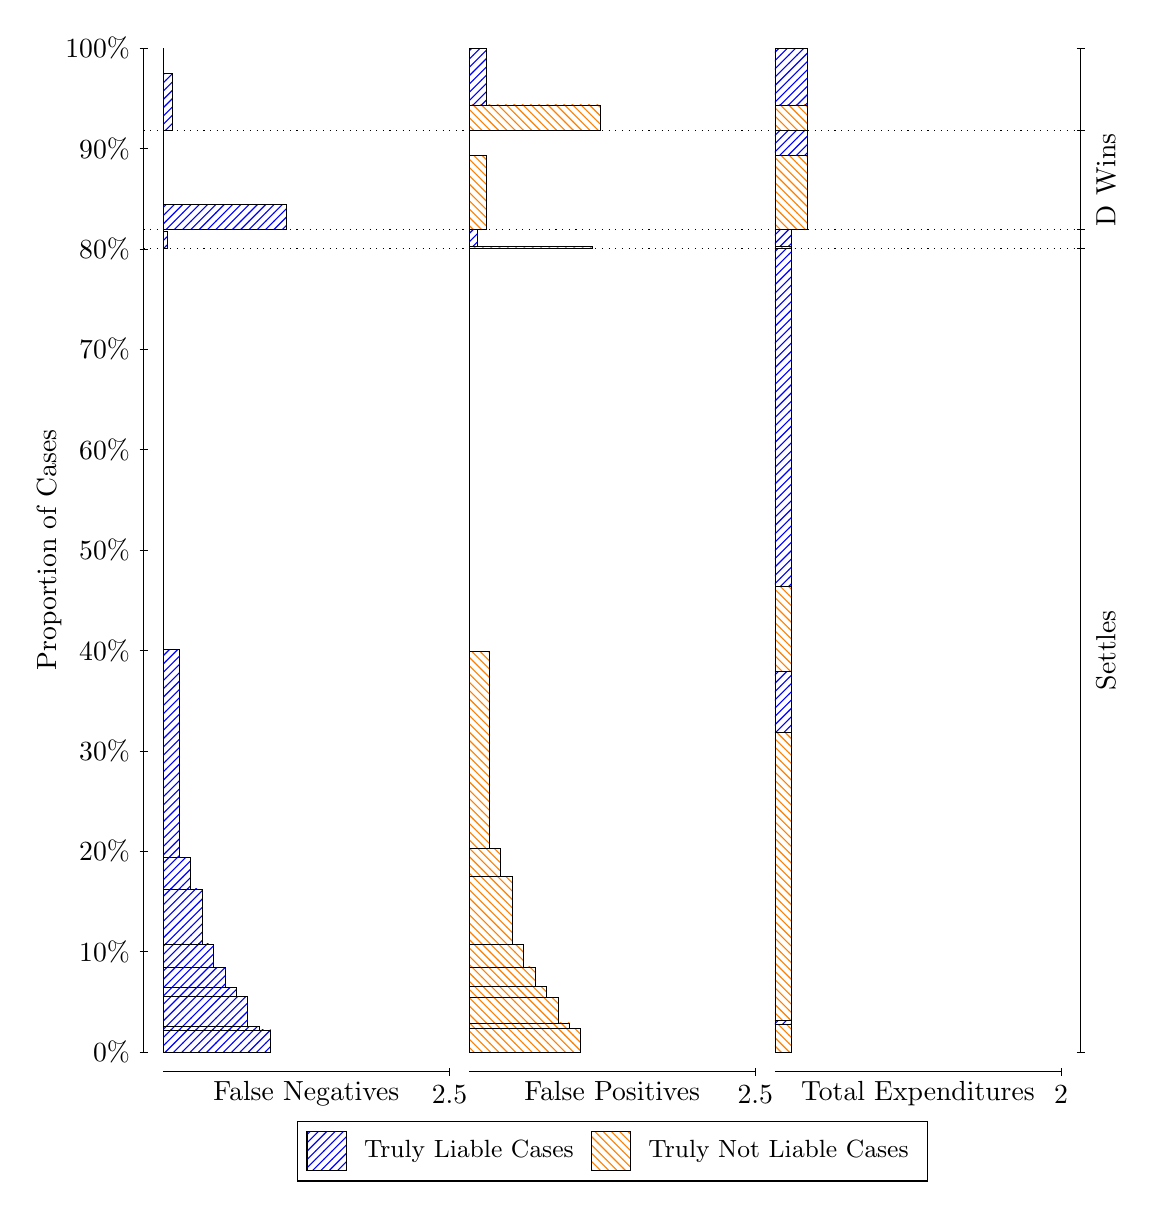
\begin{tikzpicture}
\draw[black, very thin] (1.5,1.75) -- (1.5,14.5);
\node[rotate=90, text=black, anchor=center] at (0.3, 8.125) {Proportion of Cases};
\draw[black, very thin] (1.45,1.75) -- (1.55,1.75);
\node[text=black, anchor=east] at (1.45, 1.75) {0\%};
\draw[black, very thin] (1.45,3.025) -- (1.55,3.025);
\node[text=black, anchor=east] at (1.45, 3.025) {10\%};
\draw[black, very thin] (1.45,4.3) -- (1.55,4.3);
\node[text=black, anchor=east] at (1.45, 4.3) {20\%};
\draw[black, very thin] (1.45,5.575) -- (1.55,5.575);
\node[text=black, anchor=east] at (1.45, 5.575) {30\%};
\draw[black, very thin] (1.45,6.85) -- (1.55,6.85);
\node[text=black, anchor=east] at (1.45, 6.85) {40\%};
\draw[black, very thin] (1.45,8.125) -- (1.55,8.125);
\node[text=black, anchor=east] at (1.45, 8.125) {50\%};
\draw[black, very thin] (1.45,9.4) -- (1.55,9.4);
\node[text=black, anchor=east] at (1.45, 9.4) {60\%};
\draw[black, very thin] (1.45,10.675) -- (1.55,10.675);
\node[text=black, anchor=east] at (1.45, 10.675) {70\%};
\draw[black, very thin] (1.45,11.95) -- (1.55,11.95);
\node[text=black, anchor=east] at (1.45, 11.95) {80\%};
\draw[black, very thin] (1.45,13.225) -- (1.55,13.225);
\node[text=black, anchor=east] at (1.45, 13.225) {90\%};
\draw[black, very thin] (1.45,14.5) -- (1.55,14.5);
\node[text=black, anchor=east] at (1.45, 14.5) {100\%};

\draw[black, very thin] (13.4,1.75) -- (13.4,14.5);
\draw[black, very thin] (13.35,1.75) -- (13.45,1.75);
\node[anchor=west] at (13.35, 1.75) {};
\draw[black, very thin] (13.35,11.954) -- (13.45,11.954);
\node[anchor=west] at (13.35, 11.954) {};
\draw[black, very thin] (13.35,12.197) -- (13.45,12.197);
\node[anchor=west] at (13.35, 12.197) {};
\draw[black, very thin] (13.35,13.456) -- (13.45,13.456);
\node[anchor=west] at (13.35, 13.456) {};
\draw[black, very thin] (13.35,14.5) -- (13.45,14.5);
\node[anchor=west] at (13.35, 14.5) {};

\draw[black, very thin, pattern color=blue, pattern=north east lines] (1.75,1.75) rectangle (3.1125,2.0315);
\draw[black, very thin, pattern color=blue, pattern=north east lines] (1.75,2.0315) rectangle (2.9672,2.0798);
\draw[black, very thin, pattern color=blue, pattern=north east lines] (1.75,2.0798) rectangle (2.8218,2.4521);
\draw[black, very thin, pattern color=blue, pattern=north east lines] (1.75,2.4521) rectangle (2.6765,2.5738);
\draw[black, very thin, pattern color=blue, pattern=north east lines] (1.75,2.5738) rectangle (2.5312,2.8214);
\draw[black, very thin, pattern color=blue, pattern=north east lines] (1.75,2.8214) rectangle (2.3858,3.1228);
\draw[black, very thin, pattern color=blue, pattern=north east lines] (1.75,3.1228) rectangle (2.2405,3.8219);
\draw[black, very thin, pattern color=blue, pattern=north east lines] (1.75,3.8219) rectangle (2.0952,4.2239);
\draw[black, very thin, pattern color=blue, pattern=north east lines] (1.75,4.2239) rectangle (1.9498,6.8645);
\draw[black, very thin, pattern color=orange, pattern=north west lines] (1.75,6.8645) rectangle (1.75,11.954);
\draw[black, very thin, pattern color=blue, pattern=north east lines] (1.75,11.954) rectangle (1.8045,12.17);
\draw[black, very thin, pattern color=orange, pattern=north west lines] (1.75,12.17) rectangle (1.75,12.197);
\draw[black, very thin, pattern color=blue, pattern=north east lines] (1.75,12.197) rectangle (3.3123,12.519);
\draw[black, very thin, pattern color=orange, pattern=north west lines] (1.75,12.519) rectangle (1.75,13.456);
\draw[black, very thin, pattern color=blue, pattern=north east lines] (1.75,13.456) rectangle (1.859,14.179);
\draw[black, very thin, pattern color=orange, pattern=north west lines] (1.75,14.179) rectangle (1.75,14.5);
\draw[black, very thin, pattern color=orange, pattern=north west lines] (5.6333,1.75) rectangle (7.0503,2.0475);
\draw[black, very thin, pattern color=orange, pattern=north west lines] (5.6333,2.0475) rectangle (6.905,2.1203);
\draw[black, very thin, pattern color=orange, pattern=north west lines] (5.6333,2.1203) rectangle (6.7597,2.4412);
\draw[black, very thin, pattern color=orange, pattern=north west lines] (5.6333,2.4412) rectangle (6.6143,2.5789);
\draw[black, very thin, pattern color=orange, pattern=north west lines] (5.6333,2.5789) rectangle (6.469,2.8299);
\draw[black, very thin, pattern color=orange, pattern=north west lines] (5.6333,2.8299) rectangle (6.3237,3.112);
\draw[black, very thin, pattern color=orange, pattern=north west lines] (5.6333,3.112) rectangle (6.1783,3.9807);
\draw[black, very thin, pattern color=orange, pattern=north west lines] (5.6333,3.9807) rectangle (6.033,4.3346);
\draw[black, very thin, pattern color=orange, pattern=north west lines] (5.6333,4.3346) rectangle (5.8877,6.8399);
\draw[black, very thin, pattern color=blue, pattern=north east lines] (5.6333,6.8399) rectangle (5.6333,11.954);
\draw[black, very thin, pattern color=orange, pattern=north west lines] (5.6333,11.954) rectangle (7.1957,11.981);
\draw[black, very thin, pattern color=blue, pattern=north east lines] (5.6333,11.981) rectangle (5.7423,12.197);
\draw[black, very thin, pattern color=orange, pattern=north west lines] (5.6333,12.197) rectangle (5.8513,13.134);
\draw[black, very thin, pattern color=blue, pattern=north east lines] (5.6333,13.134) rectangle (5.6333,13.456);
\draw[black, very thin, pattern color=orange, pattern=north west lines] (5.6333,13.456) rectangle (7.3047,13.778);
\draw[black, very thin, pattern color=blue, pattern=north east lines] (5.6333,13.778) rectangle (5.8513,14.5);
\draw[black, very thin, pattern color=orange, pattern=north west lines] (9.5167,1.75) rectangle (9.721,2.104);
\draw[black, very thin, pattern color=blue, pattern=north east lines] (9.5167,2.104) rectangle (9.721,2.1523);
\draw[black, very thin, pattern color=orange, pattern=north west lines] (9.5167,2.1523) rectangle (9.721,5.8083);
\draw[black, very thin, pattern color=blue, pattern=north east lines] (9.5167,5.8083) rectangle (9.721,6.5838);
\draw[black, very thin, pattern color=orange, pattern=north west lines] (9.5167,6.5838) rectangle (9.721,7.6636);
\draw[black, very thin, pattern color=blue, pattern=north east lines] (9.5167,7.6636) rectangle (9.721,11.954);
\draw[black, very thin, pattern color=orange, pattern=north west lines] (9.5167,11.954) rectangle (9.721,11.981);
\draw[black, very thin, pattern color=blue, pattern=north east lines] (9.5167,11.981) rectangle (9.721,12.197);
\draw[black, very thin, pattern color=orange, pattern=north west lines] (9.5167,12.197) rectangle (9.9254,13.134);
\draw[black, very thin, pattern color=blue, pattern=north east lines] (9.5167,13.134) rectangle (9.9254,13.456);
\draw[black, very thin, pattern color=orange, pattern=north west lines] (9.5167,13.456) rectangle (9.9254,13.778);
\draw[black, very thin, pattern color=blue, pattern=north east lines] (9.5167,13.778) rectangle (9.9254,14.5);
\draw[black, dotted] (1.5,11.954) -- (13.4,11.954);
\draw[black, dotted] (1.5,12.197) -- (13.4,12.197);
\draw[black, dotted] (1.5,13.456) -- (13.4,13.456);
\draw[black, very thin] (1.75,1.5) -- (5.3833,1.5);
\node[text=black, anchor=north] at (3.5667, 1.5) {False Negatives};
\draw[black, very thin] (5.3833,1.45) -- (5.3833,1.55);
\node[text=black, anchor=north] at (5.3833, 1.45) {2.5};

\draw[black, very thin] (5.6333,1.5) -- (9.2667,1.5);
\node[text=black, anchor=north] at (7.45, 1.5) {False Positives};
\draw[black, very thin] (9.2667,1.45) -- (9.2667,1.55);
\node[text=black, anchor=north] at (9.2667, 1.45) {2.5};

\draw[black, very thin] (9.5167,1.5) -- (13.15,1.5);
\node[text=black, anchor=north] at (11.333, 1.5) {Total Expenditures};
\draw[black, very thin] (13.15,1.45) -- (13.15,1.55);
\node[text=black, anchor=north] at (13.15, 1.45) {2};

\node[text=black, centered, rotate=90] at (13.72, 6.8522) {Settles};

\node[text=black, centered, rotate=90] at (13.72, 12.827) {D Wins};


\draw (7.449999999999999,1.5) node[draw=none] (baseCoordinate) {};
\begin{scope}[align=center]
        \matrix[scale=0.5, draw=black, below=0.5cm of baseCoordinate, nodes={draw}, column sep=0.1cm]{
            \node[rectangle, draw, minimum width=0.5cm, minimum height=0.5cm, pattern color=blue, pattern=north east lines] {}; &
            \node[draw=none, font=\small, text=black] (B) {Truly Liable Cases}; &
            \node[rectangle, draw, minimum width=0.5cm, minimum height=0.5cm, pattern color=orange, pattern=north west lines] {}; &
            \node[draw=none, font=\small, text=black] (B) {Truly Not Liable Cases}; \\
            };
\end{scope}

\end{tikzpicture}
\end{document}